% ---------------------------------------------------------------------------
% ---------------------------------------------------------------------------
% Modelo LaTex para preparação do documento final de Monografia TCC
% O modelo em conformidade com ABNT NBR
% IMT
% ---------------------------------------------------------------------------
% ---------------------------------------------------------------------------

\documentclass[
	% -- opções da classe memoir --
	12pt,					% tamanho da fonte
	openright,				% capítulos começam em pág ímpar (insere página vazia caso preciso)
	oneside,					% para impressão em verso e anverso. Oposto a oneside
	a4paper,					% tamanho do papel. 
	% -- opções da classe abntex2 --
	%chapter=TITLE,			% títulos de capítulos convertidos em letras maiúsculas
	%section=TITLE,			% títulos de seções convertidos em letras maiúsculas
	%subsection=TITLE,		% títulos de subseções convertidos em letras maiúsculas
	%subsubsection=TITLE,	% títulos de subsubseções convertidos em letras maiúsculas
    sumario=abnt-6027-2018,
	% -- opções do pacote babel --
	english,					% idioma adicional para hifenização
	%french,					% idioma adicional para hifenização
	%spanish,				% idioma adicional para hifenização
	brazil					% o último idioma é o principal do documento
	]{abntex2}

% ---------------------
% Pacotes OBRIGATÓRIOS
% ---------------------
\usepackage{lmodern}				% Usa a fonte Latin Modern			
\usepackage[T1]{fontenc}			% Selecao de codigos de fonte.
\usepackage[utf8]{inputenc}		% Codificacao do documento (conversão automática dos acentos)
\usepackage{lastpage}			% Usado pela Ficha catalográfica
\usepackage{indentfirst}		% Indenta o primeiro parágrafo de cada seção.
\usepackage{color}				% Controle das cores
\usepackage{graphicx,graphicx}	% Inclusão de gráficos
\usepackage{epsfig,subfig}		% Inclusão de figuras
\usepackage{microtype} 			% Melhorias de justificação
% ---------------------
		
% ---------------------
% Pacotes ADICIONAIS
% ---------------------
\usepackage{multirow}
\usepackage{lipsum}						% Geração de dummy text
\usepackage{amsmath,amssymb,mathrsfs}	% Comandos matemáticos avançados 
\usepackage{setspace}  					% Para permitir espaçamento simples, 1 1/2 e duplo
\usepackage{verbatim}					% Para poder usar o ambiente "comment"
\usepackage{tabularx} 					% Para poder ter tabelas com colunas de largura auto-ajustável
\usepackage{afterpage} 					% Para executar um comando depois do fim da página corrente
\usepackage{url}
\usepackage{gensymb}
% Para formatar URLs (endereços da Web)
% ---------------------

% ---------------------
% Pacotes de CITAÇÕES
% ---------------------
%\usepackage[brazilian,hyperpageref]{backref}	% Paginas com as citações na bibl
\usepackage[alf]{abntex2cite}				% Citações padrão ABNT (alfa)

%\usepackage[num]{abntex2cite}				% Citações padrão ABNT (numericas)
% ---------------------
\usepackage{float}
% Configurações de CITAÇÕES para abntex2
%% --- 
% CONFIGURAÇÕES DE PACOTES
% --- 

% ---
% Configurações do pacote backref
% Usado sem a opção hyperpageref de backref
%\renewcommand{\backrefpagesname}{Citado na(s) página(s):~}
% Texto padrão antes do número das páginas
%\renewcommand{\backref}{}
% Define os textos da citação
%\renewcommand*{\backrefalt}[4]{
%	\ifcase #1 %
%		Nenhuma citação no texto.%
%	\or
%		Citado na página #2.%
%	\else
%		Citado #1 vezes nas páginas #2.%
%	\fi}%
% ---

% Inclusão de dados para CAPA e FOLHA DE ROSTO (título, autor, orientador, etc.)
% ---
% Informações de dados para CAPA e FOLHA DE ROSTO
% ---
\titulo{Título do Trabalho...}
\autor{
    Aluno 1\\
    Aluno 2 \\
    Aluno 3 \\
    Aluno 4}

\local{São Caetano do Sul, SP}
\data{\the\year{}}
\orientador{Prof. Ms. Alexandre Harayashiki Moreira}
\instituicao{Instituto Mauá de Tecnologia - IMT}
\tipotrabalho{Trabalho de Conclusão de Curso (TCC)}

\preambulo{Trabalho de Conclusão de Curso apresentado à Escola de Engenharia Mauá do Centro Universitário do Instituto Mauá de Tecnologia como requisito parcial para a obtenção dos títulos de Engenheiro de Controle e Automação.}
% ---



% Inclui Configurações de aparência do PDF Final
%  Configurações de aparência do PDF final
% NÃO ALTERAR!!!

% alterando o aspecto da cor azul
\definecolor{blue}{RGB}{41,5,195}

% informações do PDF
\makeatletter
\hypersetup{
     	%pagebackref=true,
		pdftitle={\@title}, 
		pdfauthor={\@author},
    		pdfsubject={\imprimirpreambulo},
	    pdfcreator={LaTeX with abnTeX2},
		pdfkeywords={abnt}{latex}{abntex}{abntex2}{trabalho acadêmico}, 
		colorlinks=true,       		% false: boxed links; true: colored links
    		linkcolor=black,          	% color of internal links
    		citecolor=black,        		% color of links to bibliography
    		filecolor=magenta,      		% color of file links
		urlcolor=black,
		bookmarksdepth=4
} 
\makeatother
% --- 

% O tamanho da identação do parágrafo é dado por:
\setlength{\parindent}{0cm}
\setlength{\parskip}{0.2cm} 
% Controle do espaçamento entre um parágrafo e outro:
\setlength{\parskip}{0.2cm}  % tente também \onelineskip
\setlist[itemize]{leftmargin=1.25cm}
\setlist[enumerate]{leftmargin=1.25cm}
\usepackage{listings}
\usepackage{framed}
\usepackage{color} %use color
\definecolor{mygreen}{rgb}{0,0.6,0}
\definecolor{mygray}{rgb}{0.5,0.5,0.5}
\definecolor{mymauve}{rgb}{0.58,0,0.82}
 
%Customize a bit the look.
\lstset{ %
backgroundcolor=\color{white}, % choose the background color; you must add \usepackage{color} or \usepackage{xcolor}
basicstyle=\footnotesize, % the size of the fonts that are used for the code
breakatwhitespace=false, % sets if automatic breaks should only happen at whitespace
breaklines=true, % sets automatic line breaking
captionpos=b, % sets the caption-position to bottom
commentstyle=\color{mygreen}, % comment style
deletekeywords={...}, % if you want to delete keywords from the given language
escapeinside={\%*}{*)}, % if you want to add LaTeX within your code
extendedchars=true, % lets you use non-ASCII characters; for 8-bits encodings only, does not work with UTF-8
frame=single, % adds a frame around the code
keepspaces=true, % keeps spaces in text, useful for keeping indentation of code (possibly needs columns=flexible)
keywordstyle=\color{blue}, % keyword style
% language=Octave, % the language of the code
morekeywords={*,...}, % if you want to add more keywords to the set
numbers=left, % where to put the line-numbers; possible values are (none, left, right)
numbersep=5pt, % how far the line-numbers are from the code
numberstyle=\tiny\color{mygray}, % the style that is used for the line-numbers
rulecolor=\color{black}, % if not set, the frame-color may be changed on line-breaks within not-black text (e.g. comments (green here))
showspaces=false, % show spaces everywhere adding particular underscores; it overrides 'showstringspaces'
showstringspaces=false, % underline spaces within strings only
showtabs=false, % show tabs within strings adding particular underscores
stepnumber=1, % the step between two line-numbers. If it's 1, each line will be numbered
stringstyle=\color{mymauve}, % string literal style
tabsize=2, % sets default tabsize to 2 spaces
title=\lstname % show the filename of files included with \lstinputlisting; also try caption instead of title
}
%END of listing package%
 
\definecolor{darkgray}{rgb}{.4,.4,.4}
\definecolor{purple}{rgb}{0.65, 0.12, 0.82}
 
%define Javascript language
\lstdefinelanguage{JavaScript}{
keywords={typeof, new, true, false, catch, function, return, null, catch, switch, var, if, in, while, do, else, case, break},
keywordstyle=\color{blue}\bfseries,
ndkeywords={class, export, boolean, throw, implements, import, this},
ndkeywordstyle=\color{darkgray}\bfseries,
identifierstyle=\color{black},
sensitive=false,
comment=[l]{//},
morecomment=[s]{/*}{*/},
commentstyle=\color{purple}\ttfamily,
stringstyle=\color{red}\ttfamily,
morestring=[b]',
morestring=[b]"
}
 
\lstset{
language=JavaScript,
extendedchars=true,
basicstyle=\footnotesize\ttfamily,
showstringspaces=false,
showspaces=false,
numbers=left,
numberstyle=\footnotesize,
numbersep=9pt,
tabsize=2,
breaklines=true,
showtabs=false,
captionpos=b,
aboveskip=20pt,
belowskip=0pt,
}


\newcommand{\refanexo}[1]{\hyperref[#1]{Anexo~\ref{#1}}}


% ---------------------
% Compila o indice
% ---------------------
\makeindex
% ---------------------

%%%%%%%%%%%%%%%%%%%%%%%%%%%
%%  INICIO DO DOCUMENTO  %%
%%%%%%%%%%%%%%%%%%%%%%%%%%%
\begin{document}

% Retira espaço extra obsoleto entre as frases.
\frenchspacing

% ----------------------------------------------------------
% ELEMENTOS PRÉ-TEXTUAIS (Capa, Resumo, Abstract, etc.)
% ----------------------------------------------------------
\pretextual

% Elementos textuais com numeração arábica
\pagenumbering{arabic}

% Reinicia a contagem do número de páginas
\setcounter{page}{1}

% Capa
% ---
% Impressão da Capa
% ---
  \begin{capa}%
    \center
	\ABNTEXchapterfont\large{Centro Universitário do Instituto Mauá de Tecnologia \\Escola de Engenharia Mauá\\Engenharia de Controle e Automação}
	%\vspace{1.5cm}

    \vfill
    \ABNTEXchapterfont\bfseries\LARGE\imprimirtitulo
    \vfill

	%\vfill
	\ABNTEXchapterfont\large\imprimirautor
	\vfill
%
    \large\imprimirlocal \\
    \large\imprimirdata

    \vspace*{1cm}
  \end{capa}
% ---

% Folha de rosto (o * indica que haverá a ficha bibliográfica)
\imprimirfolhaderosto*

% Imprimir Ficha Catalografica
% ---
% Ficha Catalográfica
% ---
% Isto é um exemplo de Ficha Catalográfica, ou ``Dados internacionais de
% catalogação-na-publicação''. Você pode utilizar este modelo como referência. 
% Porém, provavelmente a biblioteca da sua universidade lhe fornecerá um PDF
% com a ficha catalográfica definitiva após a defesa do trabalho. Quando estiver
% com o documento, salve-o como PDF no diretório do seu projeto e substitua todo
% o conteúdo de implementação deste arquivo pelo comando abaixo:
%
% \begin{fichacatalografica}
%     \includepdf{fig_ficha_catalografica.pdf}
% \end{fichacatalografica}
\begin{fichacatalografica}
	\vspace*{\fill}					% Posição vertical

	\raggedleft					% Minipage Centralizado
	\fbox{\begin{minipage}[c]{12.5cm}		% Largura
	
	\hspace{0.5cm} Sobrenome, Nome do primeiro autor (citado na folha de rosto)\\
	
	\hspace{0.5cm} \imprimirtitulo  / Nome completo dos autores. --
	São Caetano do Sul: CEUN-IMT, \imprimirdata.
	
	\hspace{0.5cm} \pageref{LastPage} p.\\
	
	\hspace{0.5cm} Trabalho de Conclusão de Curso - Escola de Engenharia Mauá do Centro \\
Universitário do Instituto Mauá de Tecnologia, São Caetano do Sul, SP, \imprimirdata \\
	
	\hspace{0.5cm} \imprimirorientadorRotulo~\imprimirorientador\\

	\hspace{0.5cm}
		1. Palavra-chave1. 2. Palavra-chave2. 3. Palavra-chave3. 4. Palavra-chave4. 5. Palavra-chave5. I. Sobrenome, Nome do Segundo Autor. II. Sobrenome, Nome do Terceiro Autor. III. Sobrenome, Nome do Quarto Autor. IV. Instituto Mauá de Tecnologia. Escola de Engenharia. V. \imprimirtitulo\\
	
	\end{minipage}}
	
\end{fichacatalografica}
% ---

% ---	\hrule							% Linha horizontal
% ---	\begin{center}					% Minipage Centralizado
% ---	\begin{minipage}[c]{12.5cm}		% Largura
% ---	
% ---	\imprimirautor
% ---	
% ---	\hspace{0.5cm} \imprimirtitulo  / \imprimirautor. --
% ---	\imprimirlocal, \imprimirdata-
% ---	
% ---	\hspace{0.5cm} \pageref{LastPage} p. : il. (algumas color.) ; 30 cm.\\
% ---	
% ---	\hspace{0.5cm} \imprimirorientadorRotulo~\imprimirorientador\\
% ---	
% ---	\hspace{0.5cm}
% ---	\parbox[t]{\textwidth}{\imprimirtipotrabalho~--~\imprimirinstituicao,
% ---	\imprimirdata.}\\
% ---	
% ---	\hspace{0.5cm}
% ---		1. Palavra-chave1.
% ---		2. Palavra-chave2.
% ---		I. Orientador.
% ---		II. Universidade xxx.
% ---		III. Faculdade de xxx.
% ---		IV. Título\\ 			
% ---	
% ---	\hspace{8.75cm} CDU 02:141:005.7\\
% ---	
% ---	\end{minipage}
% ---	\end{center}
% ---	\hrule

% Inserir Folha de Aprovação
% ---
% Assinaturas
% ---
% Isto é um exemplo de Folha de aprovação, elemento obrigatório da NBR
% 14724/2011 (seção 4.2.1.3). Você pode utilizar este modelo até a aprovação
% do trabalho. Após isso, substitua todo o conteúdo deste arquivo por uma
% imagem da página assinada pela banca com o comando abaixo:
%
% \includepdf{folhadeaprovacao_final.pdf}
%
\begin{folhadeaprovacao}

  \begin{center}
    {\ABNTEXchapterfont\large\imprimirautor}

    \vspace*{\fill}\vspace*{\fill}
    \begin{center}
      \ABNTEXchapterfont\bfseries\Large\imprimirtitulo
    \end{center}
    \vspace*{\fill}
    
    \hspace{.45\textwidth}
    \begin{minipage}{.5\textwidth}
        \imprimirpreambulo
    \end{minipage}%
    \vspace*{\fill}
   \end{center}

   \assinatura{\textbf{\imprimirorientador} \\ Orientador}
   \coorientador{XXX}
   \assinatura{\textbf{\imprimircoorientador} \\ Avaliador}
   \coorientador{XXX}
   \assinatura{\textbf{\imprimircoorientador} \\ Avaliador}
   \begin{center}
    \vspace*{0.5cm}
    {\large\imprimirlocal}
    \par
    {\large\imprimirdata}
    \vspace*{1cm}
  \end{center}
  
\end{folhadeaprovacao}
% ---

% Dedicatória
%% ---
% Dedicatória
% ---
\begin{dedicatoria}
   \vspace*{\fill}
   \centering
   \noindent
   \textit{ Aos pais, amigos e familiares que nos apoiaram física e emocionalmente durante o percurso de mais uma etapa de nossas vidas.} \vspace*{\fill}
\end{dedicatoria}
% ---

% Agradecimentos
% ---
% Agradecimentos
% ---
\begin{agradecimentos}



\end{agradecimentos}
%% ---
%
% Epígrafe
% ---
% Epígrafe
% ---
\begin{epigrafe}
    \vspace*{\fill}
	\begin{flushright}
		\textit{``We can only see a short distance ahead, but we can see plenty there that needs to be done.'' \\
		          (Alan Turing)}
	\end{flushright}
\end{epigrafe}
% ---

% Resumo e Abstract
% ---
% RESUMOS
% ---

\setlength{\absparsep}{18pt} % ajusta o espaçamento dos parágrafos do resumo
\begin{resumo}
É a apresentação concisa do texto, destacando seus aspectos de maior relevância. Na elaboração do resumo, deve-se:

\begin{itemize}
    \item redigir em um único parágrafo com, no máximo, 500 palavras;
    \item redigir com frases completas e não com sequências de títulos;
    \item usar o verbo na voz ativa e na terceira pessoa do singular;
    \item evitar o uso de citações bibliográficas;
    \item ressaltar os objetivos, metodologia, resultados e conclusões do trabalho;
\end{itemize}

\textbf{Palavras-chaves}: palavras mais representativas do trabalho, separadas entre si por ponto e finalizadas também por ponto.
\end{resumo}

% ABSTRACT in english
\begin{resumo}[Abstract]
 \begin{otherlanguage*}{english}

Resumo em língua extrangeira para divulgação internacional.

   \textbf{Keywords}: X. X. X. X.
 \end{otherlanguage*}
\end{resumo}

% Lista de ilustrações
\pdfbookmark[0]{\listfigurename}{lof}
\listoffigures*
\cleardoublepage

% Lista de tabelas
%\pdfbookmark[0]{\listtablename}{lot}
%\listoftables*
%\cleardoublepage

% Lista de abreviaturas e siglas
%\begin{siglas}
%  \item[ABNT] Associação Brasileira de Normas Técnicas
%  \item[abnTeX] ABsurdas Normas para TeX
%\end{siglas}

% Lista de símbolos
%\begin{simbolos}
%  	\item[$ \vec{F_p} $] Força peso

%\end{simbolos}

%\renewcommand{\ABNTEXsectionfontsize}{\bfseries\normalsize}
%
%\renewcommand{\ABNTEXchapterfontsize}{\bfseries\Large}

% Inserir o SUMÁRIO
\pdfbookmark[0]{\contentsname}{toc}
\tableofcontents*
\cleardoublepage

% ----------------------------------------------------------
% ELEMENTOS TEXTUAIS (Capítulos)
% ----------------------------------------------------------
\textual


% Inclui cada capitulo da Dissertação
% ----------------------------------------------------------
% Introdução 
% Capítulo sem numeração, mas presente no Sumário
% ----------------------------------------------------------

\chapter{Introdução}

Introdução é a parte do trabalho em que o assunto é apresentado em sua totalidade, mas sem detalhes. Trata-se do elemento explicativo do autor para o leitor. A introdução deve:

\begin{itemize}
    \item estabelecer o assunto, definindo-o sucinta e claramente, sem deixar dúvidas quanto ao campo e período abrangidos e incluir informações sobre a natureza e importância do problema;
    \item indicar os objetivos e a finalidade do trabalho, justificar e esclarecer de que ponto de vista é tratado o assunto;
    \item referir-se aos tópicos principais do texto, dando o roteiro ou a ordem de exposição.
    \item referir-se aos tópicos principais do texto, dando o roteiro ou a ordem de exposição.
\end{itemize}

Na introdução não são mencionados os resultados alcançados, pois acarretaria desinteresse pela leitura integral do texto. É recomendável que na introdução estejam descritasa hipóteses, objeto de discussão no trabalho.

\section{Motivações e Justificativas}

\textcolor{red}{Por quê vale a pena pesquisar sobre o assunto?}

\section{Objetivos}

\textcolor{red}{Deve conter uma frase que deixe bem claro o que será desenvolvido.}

``Construção de um robô, controlado por um smartphone, capaz de ...''.

\textcolor{red}{Para facilitar o desenvolvimento do trabalho, pode-se criar objetivos específicos. Além de criar um ``fuxo de trabalho'', estes objetivos específicos auxiliam o leitor a validar se o objetivo principal foi alcançado.}

A fim de alcançar esse objetivo, alguns objetivos específicos foram definidos:
\begin{itemize}
    \item Proposta de um mecanismo para ...;
    \item Desenvolvimento de uma aplicação para ...;
    \item Montagem e testes.
\end{itemize}

\section{Organização do Trabalho}

\textcolor{red}{Como o trabalho está dividido.}

Este trabalho foi dividido em quatro grandes capítulos, com o primeiro sendo a introdução, motivação e objetivos deste trabalho. O segundo capítulo consiste em um estudo sobre... O terceiro capítulo apresenta a montagem do robô... Por fim, os resultados deste trabalho e possíveis melhorias são descritos no quarto capítulo.




% PARTE - Define a divisão do documento em partes (Não é obrigatório)
%\part{Preparação da pesquisa}
\chapter{Revisão Bibliográfica}\label{cap:estArte}

Nessa revisão deve-se conter:

\begin{itemize}
    \item fazer referências a trabalhos publicados a respeito, situando a evolução do assunto;
    \item apenas mencionar as contribuições mais importantes diretamente ligadas ao assunto;
    \item servem como base para o desenvolvimento.
\end{itemize}

\section{Como citar no Latex}

As citações podem ser diretas, quando ocorre a transcrição textual de parte da obra do autor consultado, ou indiretas, quando o texto tem base na obra do autor consultado, ou seja, o autor do trabalho cria uma paráfrase sobre as ideias dos autores consultados, com suas palavras. A paráfrase deve ser o modo principal de produção de texto na revisão da literatura.

As citações devem ser feitas de acordo com a norma e devem seguir o modelo Autor-data, em que a data é o ano. Se a citação estiver dentro de parênteses, ela deve ser destacada no texto e escrita com letras MAIÚSCULAS, se estiver fora de parênteses, deve ser escrita em letras minúsculas como segue:

\begin{itemize}
    \item único autor: Silva (2008) ou (SILVA, 2008);
    \item dois ou três autores: Tortora, Funke e Case (2000) ou  (TORTORA, FUNKE e CASE, 2000);
    \item mais de três autores: Kearney et al . (2009) ou (KEARNEY et al., 2009);
    \item No caso de haver mais de uma obra citada para o mesmo parágrafo, os autores devem aparecer em ordem ALFABÉTICA na citação, por exemplo, (CUNHA, 2009; KIRK et al., 2013; POTTER e BIRMANN , 1999; WEISS et al., 2011)
\end{itemize}

Exemplos:

De acordo com \citeonline{lu2017industry}

bla bla bla bla bla bla bla \cite{lu2017industry}

De acordo com \citeonline{sacomano2018industria}

bla bla bla bla bla bla bla \cite{sacomano2018industria}


Se a citação for textual, deve-se adicionar o número da página, como no exemplo: Segundo a NBR 10520 (2002, p. 2), "As citações diretas, no texto, de até três linhas, devem estar contidas entre aspas duplas. As aspas simples são utilizadas para indicar citação no interior de citação."

Para indicar a página utiliza-se: 

De acordo com \citeonline [p.~12] {lu2017industry} "As citações diretas, no texto, de até três linhas, devem estar contidas entre aspas duplas. As aspas simples são utilizadas para indicar citação no interior de citação."

\section{Figuras no Latex}

Ilustração é o termo genérico que abrange todo o elemento gráfico de apoio ao texto (ABNT NBR 14724, 2011). Na área técnica o termo mais comum é: \textbf{Figura}

Digamos que haja um texto e que ele seja ilustrado por uma figura. Cuidar com a expressão abaixo e acima. Usar a expressão “a seguir”, pois a figura sempre estará “a seguir” e, muitas vezes a figura “abaixo” acaba ficando “acima” na próxima página, por causa da inserção de mais texto no documento.

A forma de apresentação das ilustrações é definida pela NBR 14724 (2011) e tem a estrutura apresentada a seguir.

\begin{itemize}
    \item Título deve ficar ACIMA da figura (colocar o ponteiro do mouse sobre a figura e clicar no botão direito que aparece o comando Legenda). O título não leva ponto ao seu final;
    \item Figura propriamente dita – propriedades, dimensionamento, posicionamento (colocar o ponteiro do mouse sobre a figura e clicar no botão direito que aparecem os comandos Tamanho e posição e Formatar imagem);
    \item Fonte – logo após a figura.
\end{itemize}

\begin{figure}[h]
    \centering
    \caption{Perspectiva da superfície de Marte}
    \centering
    
\includegraphics[width=.40\linewidth]{images/latex_00.jpg}
    \caption*{Fonte: \cite{lu2017industry} }
    \label{fig:my_label}
\end{figure}

É importante esclarecer que TODOS os elementos de apoio ao texto — Figuras, Tabelas, Referências, Apêndices e Anexos — além das equações (que são elementos de texto destacados) devem ser citados no texto, ou seja, nada é inserido no trabalho sem que o texto lhe faça a devida referência. Exemplo: na Figura \ref{fig:my_label}.... Figura \ref{fig:my_label2}

\begin{figure}[h]
    \centering
    \caption{Perspectiva da superfície de Marte}
    \centering
    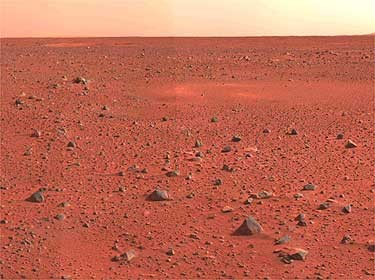
\includegraphics[width=.65\linewidth]{images/marte.jpg}
    \caption*{Fonte: Northeastern News \footnotemark , 2020}
    \label{fig:my_label2}
\end{figure}

\begin{figure}[h]
    \centering
    \caption{Perspectiva da superfície de Marte}
    \centering
    
\includegraphics[width=.40\linewidth]{images/latex_00.jpg}
    \caption*{Fonte: \cite{lu2017industry} }
    \label{fig:my_label4}
\end{figure}

\begin{figure}[h]
    \centering
    \caption{Perspectiva da superfície de Marte}
    \centering
    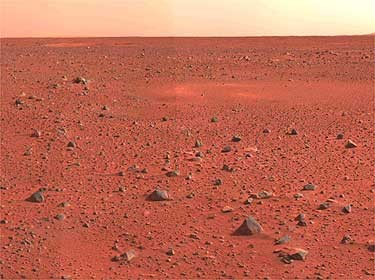
\includegraphics[width=.65\linewidth]{images/marte.jpg}
    \caption*{Fonte: Northeastern News \footnotemark , 2020}
    \label{fig:my_label3}
\end{figure}

Na Figura \ref{fig:my_label2}  e na Figura \ref{fig:my_label3} se apresenta uma sugestão para a indicação da fonte de figuras obtidas da internet. Em vez de se colocar o endereço completo (string) do qual se copiou a imagem após a palavra fonte, ele pode ser deslocado para uma nota de rodapé e, no seu lugar, se coloca a indicação do sítio no qual se encontrava a imagem. Dessa forma, o endereço da internet fica associado ao sítio pelo número da nota de rodapé, favorecendo a estética. 

\footnotetext{https://news.northeastern.edu/2019/07/17/northeastern-university-looks-back-at-the-moon-landing-50-years-later-mars-and-beyond/. Acesso em 28/05/2020}

\section{Equações no Latex}

Na Equação \ref{eq:eq1} é apresentado um exemplo de equação com apenas uma linha.

\begin{equation}
\label{eq:eq1}
        \partial \Dot{S} = \left( \frac{\partial \Dot{S} } {\partial S} \right)_0 \cdot \partial S 
\end{equation}

Na Equação \ref{eq:eq2} é apresentado um exemplo de equação com múltiplas linhas.

\begin{equation}
\label{eq:eq2}
    \begin{split}
        \partial \Dot{S} = \left( \frac{\partial \Dot{S} } {\partial S} \right)_0 \cdot \partial S \\
                         = \left( \frac{\partial \Dot{I} } {\partial S} \right)_0 \cdot \partial S \\
                         = \left( \frac{\partial \Dot{R} } {\partial I} \right)_0 \cdot \partial I
    \end{split}
\end{equation}

Na Equação \ref{eq:eq3} é apresentado um exemplo de um sistema equações com múltiplas linhas.
\begin{equation}
\label{eq:eq3}
    \begin{split}
        \begin{cases}
            \partial \Dot{S} =  \left( \frac{\partial \Dot{S} } {\partial S} \right)_0 \cdot \partial S \\
            \partial \Dot{I} = \left( \frac{\partial \Dot{I} } {\partial S} \right)_0 \cdot \partial S \\
            \partial \Dot{R} = \left( \frac{\partial \Dot{R} } {\partial I} \right)_0 \cdot \partial I
        \end{cases}
    \end{split}
\end{equation}



\chapter{Metodologia}\label{cap:metodologia}

Compreendem o instrumental empregado e a descição das técnicas adotadas e deve ser apresentada de forma cronológica em que o trabalho foi desenvolvido. Nesta seção deve-se conter:

\begin{itemize}
    \item a descrição precisa dos métodos, materiais, técnicas e equipamentos utilizados para permitir a repetição do experimento ou estudo com a mesma exatidão por outros pesquisadores;
    \item os métodos inéditos, desenvolvidos pelo autor devem ser justificados e as suas vantagens em relação a outros devem ser apontadas;
    \item os dados utilizados na análise estatística devem figurar no texto ou estar anexos ao trabalho.
\end{itemize}
\chapter{Testes e Resultados}

Devem ser elaborados testes com o objetivo de validar o funcionamento do que foi desenvolvido. Testes de repetibilidade, precisão, usabilidade, etc. 

Na análise dos resultados são apresentados os resultados obtidos de forma clara e precisa, considerando-se que:

\begin{itemize}
    \item a análise dos dados, sua interpretação e adiscussão teórica podem ser conjugados ou separados, conforme for mais adequado aos objetivos do trabalho;
    \item os diversos resultados obtidos, sem interpretações pessoais, devem vir agrupados e ordenados convenientemente, podendo eventualmente ser acompanhados de tabelas, gráficos, quadros ou figuras para maior clareza;
    \item os dados experimentais obtidos podem ser analisados e relacionados com os principais problemas que existam sobre o assunto, dando subsídios para a conclusão.
\end{itemize}
\chapter{Conclusões e Trabalhos Futuros}

É a recapitulação sintética dos resultados e da discussão do estudo ou da pesquisa. Pode apresentar deduções lógicas e correspondentes aos objetivos propostos, ressaltando-se o alcance e as consequências de suas contribuições, bem como possível mérito. Pode conter a indicação de problemas dignos de novos estudos, além de recomendações, quando for o caso.


% ----------------------------------------------------------
% ELEMENTOS PÓS-TEXTUAIS (Referências, Glossário, Apêndices)
% ----------------------------------------------------------
%\postextual

% Referências bibliográficas
\bibliography{bibliografia}

% Glossário (Consulte o manual)
%\glossary

% Apêndices
% ----------------------------------------------------------
% Apêndices
% ----------------------------------------------------------

% ---
% Inicia os apêndices
% ---
\begin{apendicesenv}

% Imprime uma página indicando o início dos apêndices
\begin{KeepFromToc}
\partapendices*
\end{KeepFromToc}

Apendices são materiais complementares que só devem ser inclusos quando forem imprescindíveis à compreensão do texto, elaborados pelo autor a fim de completar sua argumentação. São identificados por letras maiúsculas consecutivas, travessão e pelos respectivos títulos, devendo iniciar-se em folha própria.

\end{apendicesenv}
% ---

% Anexos
% ----------------------------------------------------------
% Apêndices
% ----------------------------------------------------------

% ---
% Inicia os anexos
% ---
\begin{anexosenv}

% Imprime uma página indicando o início dos anexos
\begin{KeepFromToc}
\partanexos
\end{KeepFromToc}

Anexos são documentos não elaborados pelo autor, que servem de fundamentação, comprovação ou ilustração, como mapas, leis, estatutos, entre outros. São identificados por letras maiúsculas consecutivas, travessão e pelos respectivos títulos, devendo iniciar-se em folha própria.

\end{anexosenv}

% Índice remissivo (Consultar manual)
%\phantompart
%\printindex

\end{document}
